\chapter{实验}
\label{chapter: exp}
本章将介绍本文中为了验证方法有效性所进行的一系列实验。首先将介绍本文使用的几个公开或提出的数据集、评价指标,此后分别介绍在混合隐式场景重建、真实场景数据下实验以及场景图重建实验。除了与基线模型对比,本文还将进行一系列消融实验以验证本文方法中各个组件的有效性。


\section{数据集}
\subsection{公开数据集}
本节中介绍本文使用的公开数据集。
\subsubsection{NeuralRGB-D数据}
NeuralRGB-D\cite{azinovic_neural_2022}提出了一个基于仿真的室内场景数据集,其中包含RGB和深度的准确数据。该数据提供了在 10 个合成场景的数据集,这些场景的真实几何和相机轨迹是已知的,因此可以提供隐式场方法的定量评估指标。其中,真实相机轨迹仅用于渲染和评估,而不用于重建。对于每一帧,作者使用 Blender渲染照片般逼真的图像,其后应用噪声和伪影,来模拟类似于真实深度传感器\cite{zabatani_intel_2020, zhang_microsoft_2012}。

\begin{figure}[ht]
    \centering
    \includegraphics[width=0.6\textwidth]{undergraduate-thesis/images/experiments/neural-rgbd dataset.png}
    \caption{NeuralRGB-D\cite{azinovic_neural_2022}中的场景thin-Geometry示例图片}
    \label{fig:exp-neural-rgbd-data}
\end{figure}

\begin{figure}[ht]
    \centering
    \includegraphics[width=0.8\textwidth]{undergraduate-thesis/images/experiments/kitti-map.png}
    \caption{KITTI数据集所覆盖的地图范围}
    \label{fig:exp-kitti-map}
\end{figure}

\subsubsection{KITTI数据集}
KITTI数据集\cite{geiger_are_2012,geiger_vision_2013}是在德国卡尔斯鲁厄及其周边地区行驶时从移动平台\ref{fig:exp-kitti-platform}记录的。它包括来自组合 GPS/IMU 系统的相机图像、激光扫描、高精度 GPS 测量和 IMU 加速度。该数据集的主要目的是推动以自动驾驶为目标的计算机视觉和机器人算法的发展。在本文中使用其中包含动态物体较多的片段,以验证本文所提出的场景图方法在重建复杂动态场景时的性能。
\begin{figure}[ht]
    \centering
    \includegraphics[width=0.8\textwidth]{undergraduate-thesis/images/experiments/kitti-platform.png}
    \caption{KITTI数据集的采集平台}
    \label{fig:exp-kitti-platform}
\end{figure}

图\ref{fig:exp-kitti-map}显示了KITTI数据集在德国卡尔斯鲁厄大都市区记录的 GPS 轨迹。颜色编码 GPS 信号质量:红色表示已使用 RTK 校正以最高精度记录,蓝色表示没有校正信号。由于没有可用的 GPS 信号,黑色部分已从数据集中排除。
KITTI数据集中提供了场景中动态物体的边界框位姿,如图\ref{fig:exp-kitti-objpose}所示。对于参考相机视野内的每个动态对象,KITTI以 3D 边界框轨迹的形式提供标注,以 Velodyne 坐标表示。数据集中定义了“汽车”、“货车”、“卡车”、“行人”、“人(坐着的)”、“骑自行车的人”、“电车”和“其他”(例如拖车)等多个物体类别。

\begin{figure}[ht]
    \centering
    \includegraphics[width=\textwidth]{undergraduate-thesis/images/experiments/kitti-objects.png}
    \caption{KITTI中动态物体轨迹位姿标定可视化}
    \label{fig:exp-kitti-objpose}
\end{figure}



\subsection{本文提出的数据集}
\subsubsection{异步城市场景数据集 AUS}
本文提出异步城市场景 (AUS) 数据集。 AUS 数据集是从模拟器生成的,通过加载场景模型,模拟器可以创建模拟真实世界异步序列的异步 RGB-D 序列。该数据集由 2 个真实场景和 4 个虚拟场景组成。前者使用 Kirill Sibiriakov \cite{ArtStation}提供的纽约和旧金山城市场景,其中 AUS-NewYork 覆盖了 250×150m$^2$ 的区域,其中包含许多详细的建筑物,AUS-SanFrancisco 由金门大桥附近的 500×250m$^2$ 区域组成,而后者使用 UrbanScene3D 数据集 \cite{lin_capturing_2022} 中提供的仿真模型文件。本文利用 Unreal Engine 的物理引擎和 AirSim\cite{shah_airsim_2017}对物理属性进行建模,并使用三种类型的轨迹,包括 Zig-Zag 轨迹、更复杂的计划随机轨迹和复杂的手动控制轨迹。在虚拟场景中,因为场景尺寸相对较小,只提供手动控制的轨迹。

\begin{figure}[ht]
    \centering
    \includegraphics[width=\textwidth]{undergraduate-thesis/images/experiments/Dataset-city.pdf}
    \caption{本文提出的AUS数据集}
    \label{fig:exp-aus-dataset}
\end{figure}

在真实场景中,RGB 相机和 LiDAR 通常不会对齐,因此本文在模拟器中以高频率(50fps)对原始 RGB-D 序列进行采样,并使用不同的起始帧对其进行重新采样,以获得逼真的异步 RGB-D 序列.为了进一步增加真实性,本文向固定偏移量添加了随机扰动。采样方法如图\ref{fig:exp-aus-offset}所示。

如图\ref{fig:exp-rgbd-alignment}所示,RGB相机和深度相机在一次飞行中覆盖了几乎相同的轨迹,因此轨迹先验可以在RGB序列中隐式学习,并可以直接转换为预测深度相机位姿。
\begin{figure}[ht]
    \centering
    \includegraphics[width=0.4\textwidth]{undergraduate-thesis/images/time-pose function/RGBD_alignment.pdf}
    \caption{RGB和深度序列轨迹的可视化演示。}
    \label{fig:exp-rgbd-alignment}
\end{figure}

\begin{figure}[ht]
    \centering
    \includegraphics[width=\textwidth]{undergraduate-thesis/images/experiments/offset.pdf}
    \caption{采样策略的可视化演示。本文从每 5 帧原始 RGB-D 数据中采样一个 RGB 帧。本文通过向 RGB 帧时间戳添加不同的偏移量来计算深度帧采样时间。 AUS 数据集中包含两种类型的偏移量:(1) 两个相邻 RGB 帧之间时间间隔的 10\%-50\% 的固定偏移量(总共 5 条迹线); (2) 不固定的随机偏移量。}
    \label{fig:exp-aus-offset}
\end{figure}

\subsubsection{带雾数据集}
\textbf{真实世界数据集}:
为了评估去雾效果,本文使用无雾的真实图像数据集,并对图像进行后处理以在其上添加雾天效果。本文使用 DJI M300 无人机(配备高清 RGB 相机和 LiDAR,如图 \ref{fig:real-world-setting} 所示)来收集真实数据,其中 RGB 相机收集以 30fps 的帧速率拍摄图像,LiDAR 以 240Hz 的频率收集深度信息。 RGB 图像的位姿由机载 RTK 或 COLMAP 提供。由于大疆只在RGB EXIF信息中存储了无人机位姿数据。相比之下,激光雷达信息不携带姿态信息,本文使用Time-Pose Function来计算相应的姿态。
传感器之间的固定转换由生产商提供,也可以手动校准。本文在获取的数据集上训练 NeRFacto ~\cite{tancik_nerfstudio_2023} 模型以获得逐像素深度值,并将它们代入散射方程中以获得场景中的带雾图像。真实世界数据集的像素深度图不是通过实际测量获得的,因此没有为真实世界数据集提供可靠的几何测量数据。因此,本文只对合成数据集进行数值评估。

\begin{figure}[ht]
	\begin{center}
	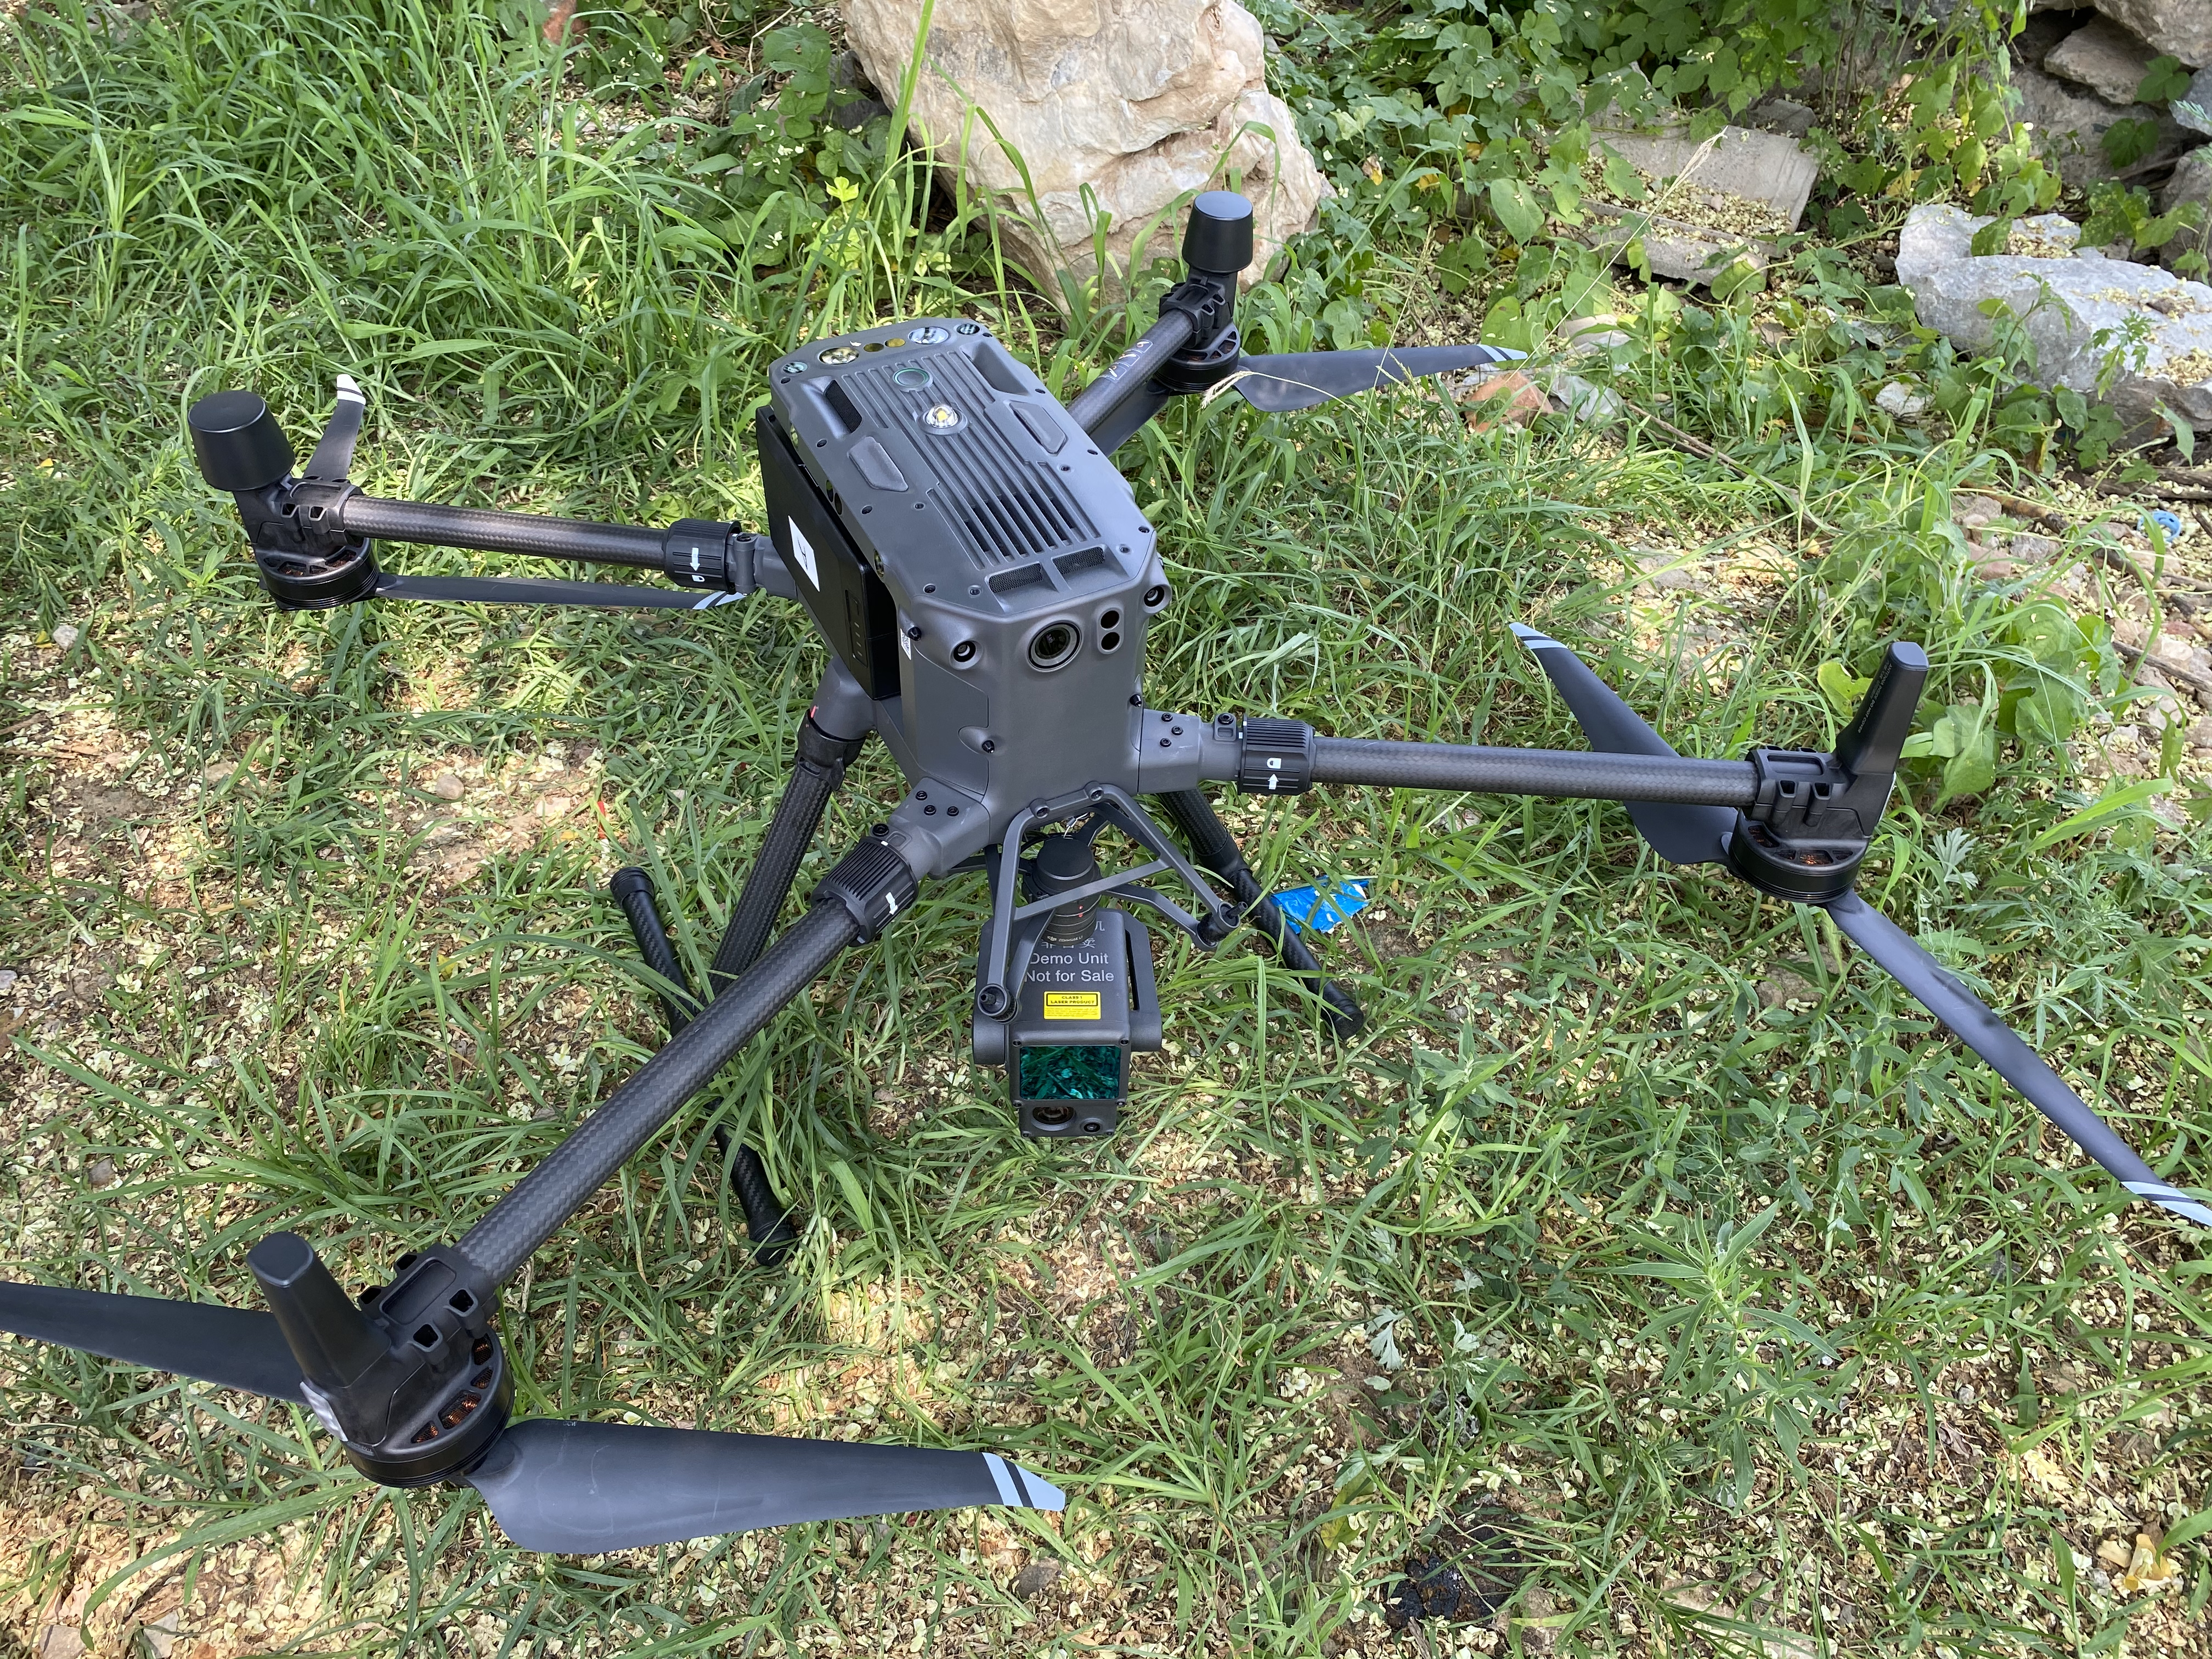
\includegraphics[width=0.3\textwidth]{undergraduate-thesis/images/experiments/aircraft.jpg}
	\includegraphics[width=0.3\textwidth]{undergraduate-thesis/images/experiments/flight-near.jpg}
	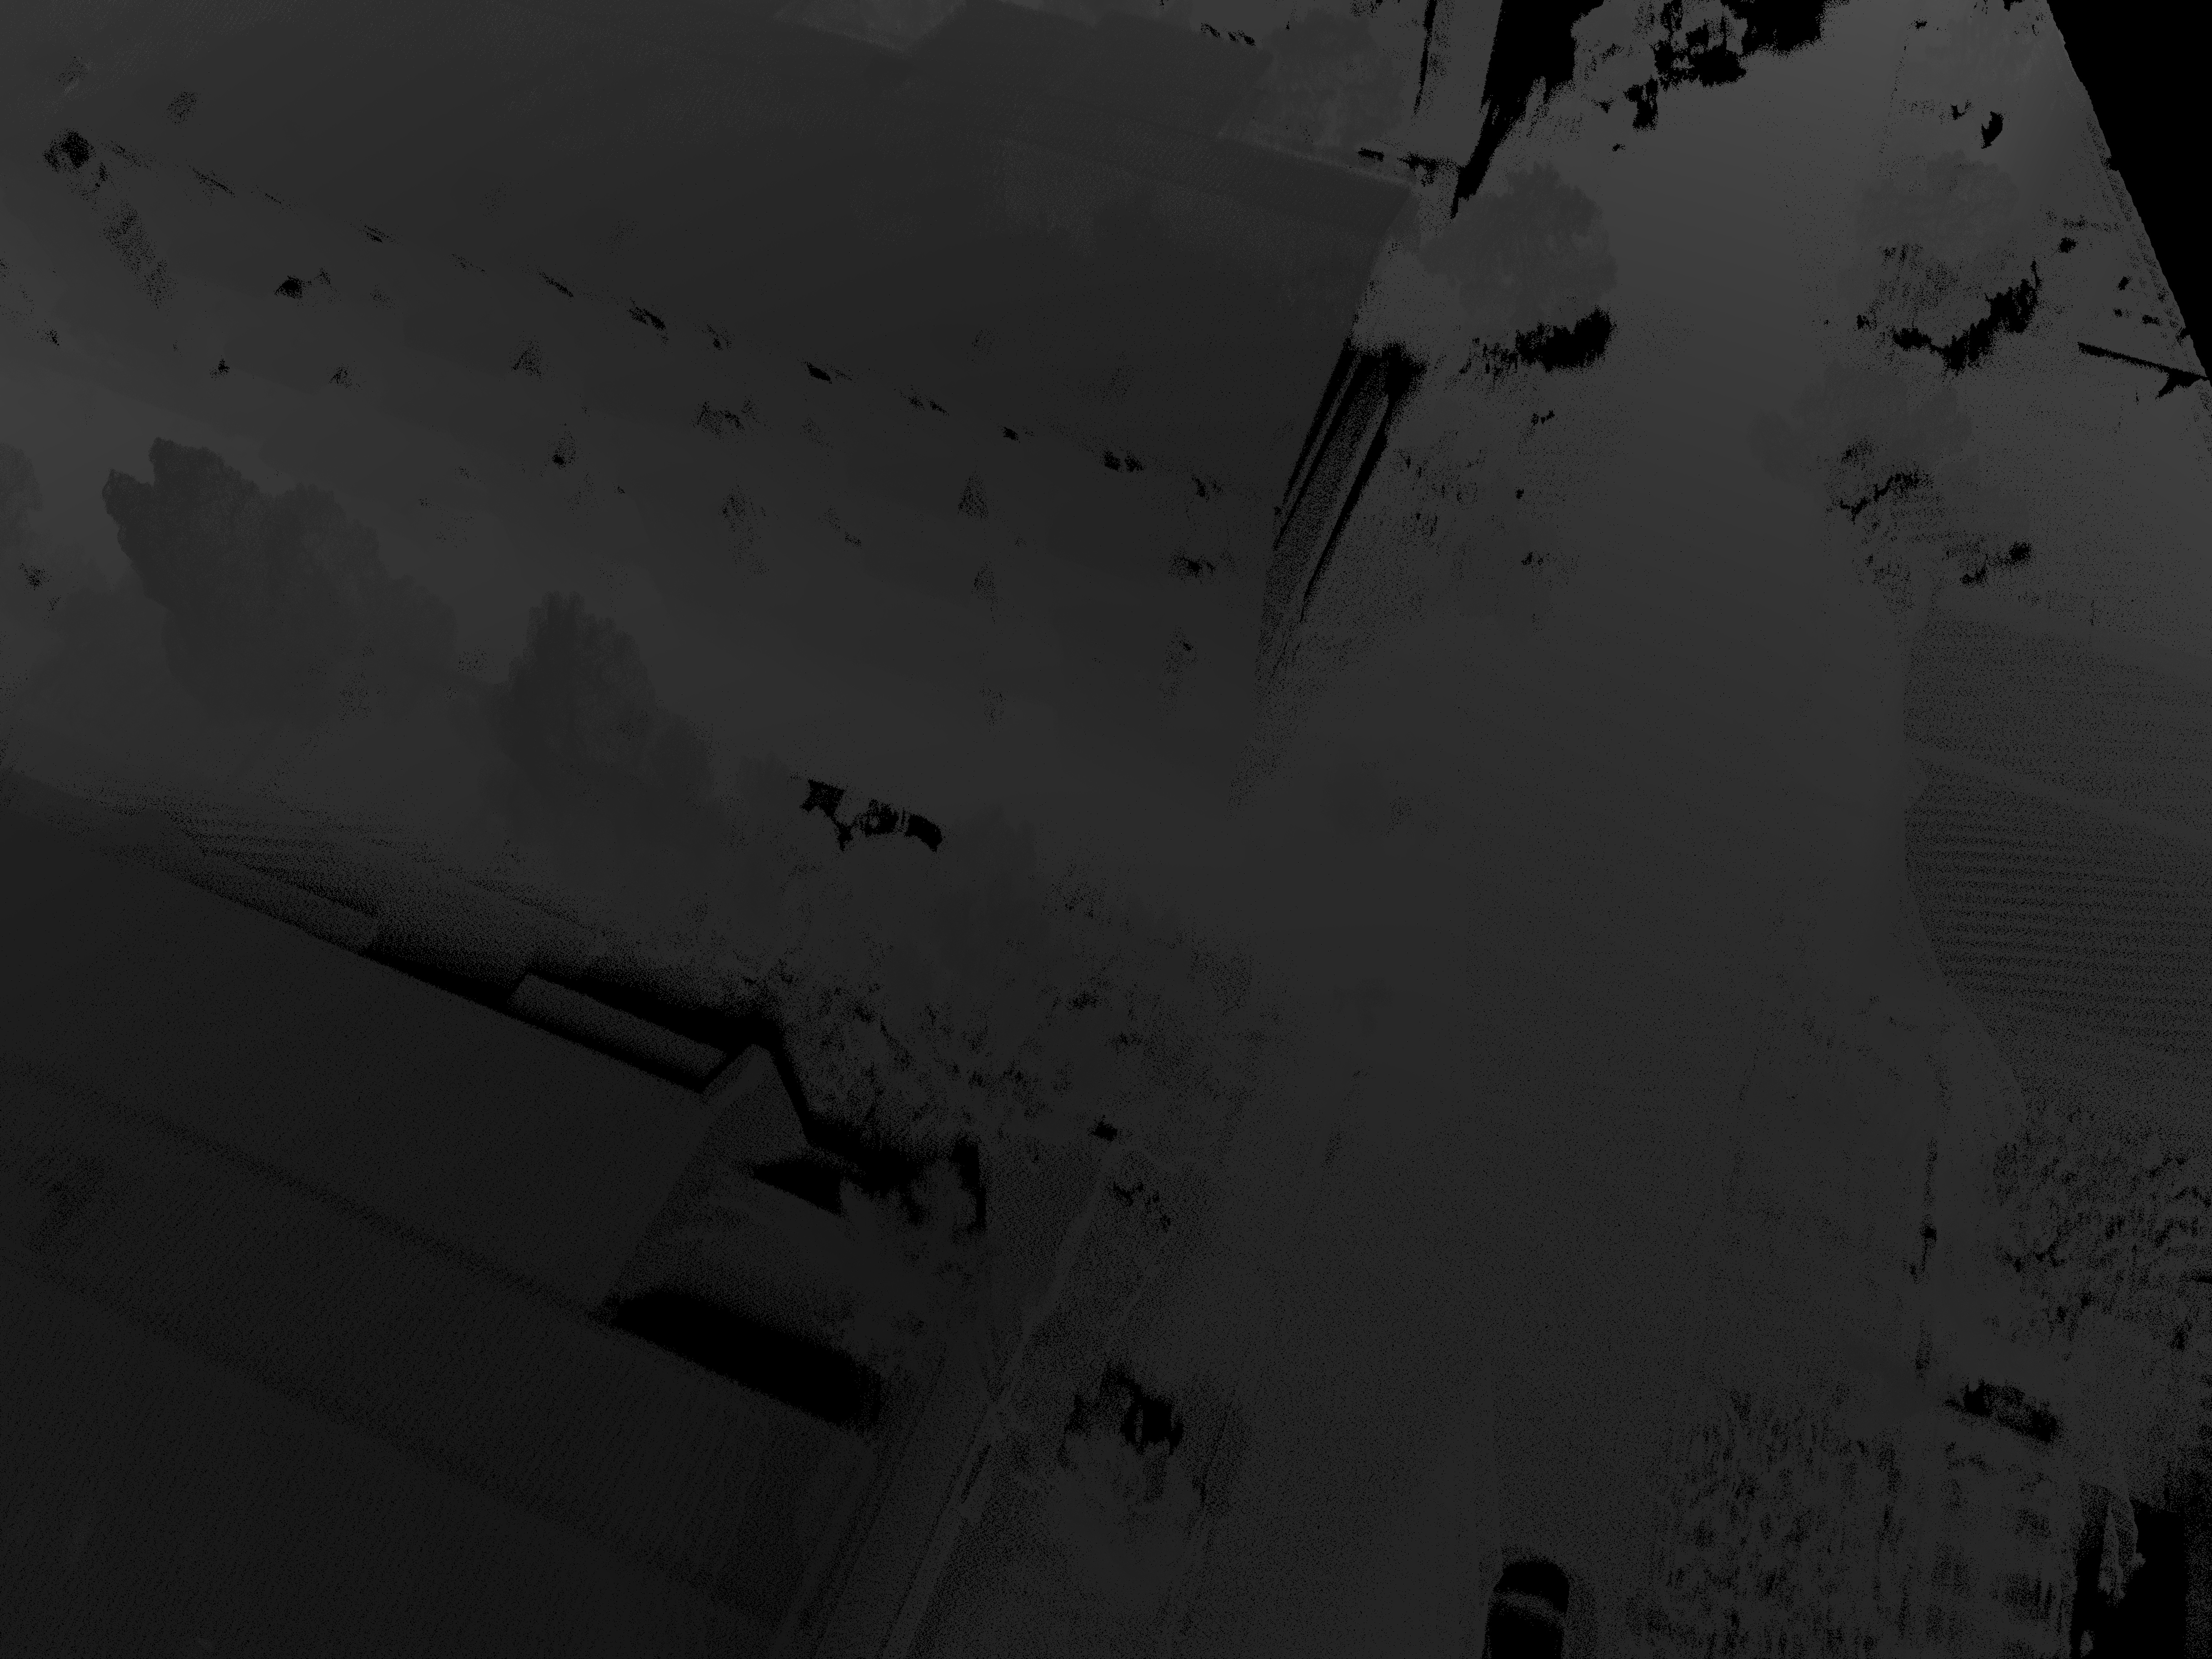
\includegraphics[width=0.3\textwidth]{undergraduate-thesis/images/experiments/pointcloud.jpg}
	\end{center}
	\caption{左图为实验中使用的无人机系统; 中间为数据采集过程中的无人机照片;右图为匹配后的点云。}
	\label{fig:real-world-setting}
\end{figure}

\textbf{合成数据集}:
本文在AUS数据集的基础上,根据数据集本身的深度信息进行带雾数据合成。该数据集提供了无雾的 RGB 图像、像素深度图和来自多个视图的相机位姿。来自相同视图的带雾图像的计算类似于真实世界数据集。不同于真实世界数据集,这个合成数据集的真实深度图被用于数值评估。

\section{混合隐式场景重建}
\subsection{实现细节}
在实验中,本文维护一个 L = 2 的多分辨率特征网格,将来自不同网格层的插值特征向量连接在一起,并通过 5 层的浅层 MLP 进行处理,其中MLP中每层有 1024 个神经元。网格的每一层使用空间哈希函数为 $h^{(l)}(x) = \left\lfloor x\right\rfloor \oplus \pi_l\ \text{mod}\ N_l$,其中 $\oplus$ 表示逐位异或运算,$N_l$ 是第 $l$ 层特征向量的数量,$π_l$ 是选定的大质数,在实验中被设置为 $\pi_0 = 1, \pi_1 = 2,654,435, 761$。

所有模型均进行了 500K 次迭代,并在每一步渲染一组 1024 条射线,场景表示网络的学习率从最开始的 $5\times10^{-4}$ 衰减到 $5\times10^{-5}$,位姿优化组件学习率由$1\times10^{-6}$ 衰减到 $1\times10^{-7}$。

\subsection{评价指标}
本文使用RGB渲染和深度预测的标准预测指标来评估所提出方法的有效性。
\subsubsection{RGB渲染}
在视角合成上,本文使用PSNR (Peak Signal-to-Noise Ratio) 峰值信噪比\cite{hore_image_2010}、结构相似度SSIM (Structural SIMilarity)\cite{hore_image_2010}以及学习感知图像块相似度(Learned Perceptual Image Patch Similarity, LPIPS)\cite{zhang_unreasonable_2018}。

给定大小为$m\times n$的原图$I$和噪声图像$K$,峰值信噪比PSNR被定义为:
\begin{equation}
    PSNR =  10\log_{10}(\frac{(2^B-1))^2}{\frac{1}{m\times n}\sum_i\sum_j(I-K)^2}),
\end{equation}
$B$为图像位数,本文使用$B=8$。

SSIM公式基于样本$x$和$y$之间的三个比较衡量:亮度 (luminance)、对比度 (contrast) 和结构 (structure):
\begin{align}
    l(x,y) &= \frac{2\mu_x\mu_y+c_1}{\mu_x^2+\mu_y^2+c_1}\\
    c(x,y) &= \frac{2\sigma_x\sigma_y+c_2},{\sigma_x^2+\sigma_y^2+c_2},\\
    s(x,y) &= \frac{\sigma_{xy}+c_3}{\sigma_x\sigma_y+c_3},
\end{align}
其中$\mu_{\{x,y\}}$为均值,$\sigma_{\{x,y\}}^2$为方差,$\sigma_{xy}$为协方差。
\begin{equation}
    SSIM(x,y) = [l(x,y)^\alpha\cdot c(x,y)^\beta\cdot s(x,y)^\gamma],
\end{equation}
$\alpha, \beta, \gamma$为超参数,本文中均设置为1。

学习感知图像块相似度(Learned Perceptual Image Patch Similarity, LPIPS)\cite{zhang_unreasonable_2018}也称为“感知损失”(perceptual loss),用于度量两张图像之间的差别。该度量标准学习生成图像到真实图像的反向映射强制生成器学习从假图像中重构真实图像的反向映射,并优先处理它们之间的感知相似度。LPIPS 比传统方法(比如L2/PSNR, SSIM, FSIM)更符合人类的感知情况。LPIPS的值越低表示两张图像越相似,反之,则差异越大。

\subsubsection{场景几何深度预测}
本文中使用的深度评估指标\cite{wang_regularizing_2021}包含Abs. Rel, Sq. Rel, RMSE, RMSE $\log$, $\delta_{\{1,2,3\}}$,其计算方法如下所示:
\begin{align}
    \text{Abs. Rel} &= \frac{1}{|D|}\sum_{d\in D} |d - \hat{d}| / d,\\
    \text{Sq. Rel} &= \frac{1}{|D|}\sum_{d\in D} ||d - \hat{d}||^2 / d,\\
    \text{RMSE} &= \sqrt{\frac{1}{|D|}\sum_{d\in D} ||d - \hat{d}||^2},\\
    \text{RMSE} \log &= \sqrt{\frac{1}{|D|}\sum_{d\in D} ||\log d - \log\hat{d}||^2},\\
    \delta_i &= \frac{1}{|D|}|\{d\in D | \max(\frac{d}{\hat{d}}, \frac{\hat{d}}{d}) < 1.25^i\}|.
\end{align}

% Please add the following required packages to your document preamble:
% \usepackage{graphicx}
\begin{table}[p]
\resizebox{\textwidth}{!}{%
\begin{tabular}{ccccccc}
\hline
场景    & \multicolumn{3}{c}{NY Simple}               & \multicolumn{3}{c}{NY Hard}                \\ \cline{2-7} 
方法    & NeRF-W  & Mega-NeRF       & Ours            & NeRF-W & Mega-NeRF       & Ours            \\ \hline
PSNR $\uparrow$  & 23.06   & 23.48           & \textbf{24.77}  & 22.88  & 23.09           & \textbf{23.99}  \\
SSIM $\uparrow$  & 0.7946  & 0.8744          & \textbf{0.8469} & 0.7899 & 0.786           & \textbf{0.8162} \\
LPIPS $\downarrow$ & 0.2318  & 0.1738          & \textbf{0.1661} & 0.2574 & 0.2339          & \textbf{0.2218} \\ \hline
场景    & \multicolumn{3}{c}{NY Manual}               & \multicolumn{3}{c}{SF Simple}              \\ \cline{2-7} 
方法    & NeRF-W  & Mega-NeRF       & Ours            & NeRF-W & Mega-NeRF       & Ours            \\ \hline
PSNR $\uparrow$  & 22.88   & 24.03           & \textbf{24.24}  & 22.12  & 19.99           & \textbf{22.7}   \\
SSIM $\uparrow$  & 0.7899  & \textbf{0.8522} & 0.8406          & 0.8297 & 0.8294          & \textbf{0.8336} \\
LPIPS $\downarrow$ & 0.2574  & 0.1683          & \textbf{0.1621} & 0.2528 & 0.2252          & \textbf{0.2067} \\ \hline
场景    & \multicolumn{3}{c}{SF Hard}                 & \multicolumn{3}{c}{SF Manual}              \\ \cline{2-7} 
方法    & NeRF-W  & Mega-NeRF       & Ours            & NeRF-W & Mega-NeRF       & Ours            \\ \hline
PSNR $\uparrow$  & 17.17   & 19.77           & \textbf{20.49}  & 18.33  & 21.83           & \textbf{23.24}  \\
SSIM $\uparrow$  & 0.5564  & 0.7112          & \textbf{0.7164} & 0.5968 & 0.6596          & \textbf{0.8291} \\
LPIPS $\downarrow$ & 0.4489  & \textbf{0.3302} & 0.3344          & 0.3878 & \textbf{0.2304} & 0.245           \\ \hline
场景    & \multicolumn{3}{c}{Bridge}                  & \multicolumn{3}{c}{Town}                   \\ \cline{2-7} 
方法    & NeRF-W  & Mega-NeRF       & Ours            & NeRF-W & Mega-NeRF       & Ours            \\ \hline
PSNR $\uparrow$  & 26.79   & 27.98           & \textbf{29.06}  & 21.32  & 24.69           & \textbf{25.32}  \\
SSIM $\uparrow$  & 0.8053  & 0.8674          & \textbf{0.8751} & 0.6208 & 0.7305          & \textbf{0.7675} \\
LPIPS $\downarrow$ & 0.2438  & \textbf{0.1548} & 0.1952          & 0.4088 & 0.3103          & \textbf{0.2631} \\ \hline
场景    & \multicolumn{3}{c}{School}                  & \multicolumn{3}{c}{Castle}                 \\ \cline{2-7} 
方法    & NeRF-W  & Mega-NeRF       & Ours            & NeRF-W & Mega-NeRF       & Ours            \\ \hline
PSNR $\uparrow$  & 19.69   & 25.57           & \textbf{26.51}  & 22.63  & 28.06           & \textbf{28.21}  \\
SSIM $\uparrow$  & 0.5715  & 0.7739          & \textbf{0.7971} & 0.7443 & \textbf{0.9053} & 0.8976          \\
LPIPS $\downarrow$ & 0.44527 & 0.3191          & \textbf{0.3175} & 0.2557 & 0.1159          & \textbf{0.1113} \\ \hline
\end{tabular}%
}
\caption{在AUS数据集的重建结果的数值评估}
\label{tab: aus-nvs-quant}
\end{table}

% Please add the following required packages to your document preamble:
% \usepackage{multirow}
% \usepackage{graphicx}
\begin{table}[p]
\caption{AUS数据集上的深度预测的数值评估结果}
\label{tab:aus-depth-quant}
\resizebox{\textwidth}{!}{%
\begin{tabular}{ccccccc}
\hline
场景                         & 方法        & RMSE $\downarrow$           & RMSE $\log\  \downarrow$       & $\delta_1\ \uparrow$            & $\delta_2\ \uparrow$            & $\delta_3\ \uparrow$            \\ \hline
\multirow{3}{*}{NY Simple} & NeRF-W    & 16.74          & 0.2149          & 84.62\%          & 93.99\%          & 99.68\%          \\
                           & Mega-NeRF & 19.74          & 0.2411          & 82.76\%          & 93.25\%          & 96.71\%          \\
                           & Ours      & \textbf{5.50}   & \textbf{0.069}  & \textbf{97.78\%} & \textbf{99.39\%} & \textbf{99.85\%} \\ \hline
\multirow{3}{*}{NY Hard}   & NeRF-W    & 9.97           & 0.2027          & 86.04\%          & 94.63\%          & 97.31\%          \\
                           & Mega-NeRF & 10.07          & 0.2117          & 87.59\%          & 95.64\%          & 97.47\%          \\
                           & Ours      & \textbf{7.03}  & \textbf{0.1672} & \textbf{94.91\%} & \textbf{97.21\%} & \textbf{98.33\%} \\ \hline
\multirow{3}{*}{NY Manual} & NeRF-W    & 25.48           & 0.3715          & 69.85\%          & 81.71\%          & 87.18\%          \\
                           & Mega-NeRF & 42.15          & 0.43            & 69.99\%          & 77.43\%          & 84.43\%          \\
                           & Ours      & \textbf{5.93}  & \textbf{0.0085} & \textbf{91.85\%} & \textbf{98.08\%} & \textbf{99.48\%} \\ \hline
\multirow{3}{*}{SF Simple} & NeRF-W    & 31.12          & 0.1988          & 86.14\%          & 90.59\%          & 98.17\%          \\
                           & Mega-NeRF & 32.17          & 0.2188          & 86.38\%          & 92.12\%          & 95.04\%          \\
                           & Ours      & \textbf{7.26}  & \textbf{0.0669} & \textbf{97.97\%} & \textbf{99.30\%} & \textbf{99.72\%} \\ \hline
\multirow{3}{*}{SF Hard}   & NeRF-W    & 23.58          & 0.1429          & 81.14\%          & 91.36\%          & 96.34\%          \\
                           & Mega-NeRF & 26.02          & 0.1666          & 86.20\%          & 94.92\%          & 96.45\%          \\
                           & Ours      & \textbf{9.99}  & \textbf{0.0992} & \textbf{93.68\%} & \textbf{97.78\%} & \textbf{99.72\%} \\ \hline
\multirow{3}{*}{SF Manual} & NeRF-W    & 20.09          & 0.2214          & 78.14\%          & 92.67\%          & 96.29\%          \\
                           & Mega-NeRF & 12.48          & 0.1286          & 93.17\%          & 97.18\%          & 99.01\%          \\
                           & Ours      & \textbf{5.66}  & \textbf{0.0706} & \textbf{97.37\%} & \textbf{99.31\%} & \textbf{99.67\%} \\ \hline
\multirow{3}{*}{Bridge}    & NeRF-W    & 131.88         & 1.2277          & 53.76\%          & 61.57\%          & 58.98\%          \\
                           & Mega-NeRF & 120.41         & 1.3246          & 69.10\%          & 72.54\%          & 73.17\%          \\
                           & Ours      & \textbf{26.56} & \textbf{0.3248} & \textbf{93.24\%} & \textbf{96.32\%} & \textbf{98.26\%} \\ \hline
\multirow{3}{*}{Town}      & NeRF-W    & 132.70          & 1.4600           & 44.89\%          & 55.68\%          & 57.90\%          \\
                           & Mega-NeRF & 129.50          & 1.4201           & 54.54\%          & 59.18\%          & 57.90\%          \\
                           & Ours      & \textbf{15.61} & \textbf{0.4632} & \textbf{91.92\%} & \textbf{96.89\%} & \textbf{98.49\%} \\ \hline
\multirow{3}{*}{School}    & NeRF-W    & 88.83          & 0.9365          & 61.73\%          & 72.58\%          & 75.80\%          \\
                           & Mega-NeRF & 63.10           & 0.7651          & 77.18\%          & 85.02\%          & 86.69\%          \\
                           & Ours      & \textbf{21.19} & \textbf{0.2083} & \textbf{92.87\%} & \textbf{95.78\%} & \textbf{97.51\%} \\ \hline
\multirow{3}{*}{Castle}    & NeRF-W    & 78.18          & 0.8651          & 75.72\%          & 79.26\%          & 81.11\%          \\
                           & Mega-NeRF & 54.99          & 0.6167          & 79.69\%          & 83.59\%          & 87.43\%          \\
                           & Ours      & \textbf{16.66} & \textbf{0.3565} & \textbf{93.12\%} & \textbf{97.23\%} & \textbf{98.45\%} \\ \hline
\end{tabular}%
}
\end{table}

\begin{table}[ht]
\centering
\resizebox{0.75\textwidth}{!}{%
\begin{tabular}{lllll}
\hline
\multicolumn{1}{c}{\multirow{2}{*}{场景}} & \multicolumn{2}{c}{TPF} & \multicolumn{2}{c}{位姿优化} \\ \cline{2-5} 
\multicolumn{1}{c}{} & 旋转 $(^\circ)$    & 平移 $(m)$    & 旋转    $(^\circ)$   & 平移  $(m)$    \\ \hline
NY Simple            & 0.6601 & 1.84   & 0.1336 & 0.3394 \\
NY Hard              & 0.5908 & 1.12   & 0.089  & 0.5644 \\
NY Manual            & 3.698  & 0.4605 & 1.474  & 0.1997 \\
SF Simple            & 0.17   & 1.338  & 0.0465 & 0.3193 \\
SF Hard              & 0.6656 & 1.4488 & 0.4064 & 1.088  \\
SF Manual            & 0.6539 & 0.9393 & 0.0191 & 0.6632 \\
Bridge               & 1.5108 & 0.9514 & 0.4893 & 0.5709 \\
Town                 & 0.6774 & 1.346  & 0.3633 & 0.8463 \\
School               & 0.7031 & 0.878  & 0.6807 & 0.56   \\
Castle               & 1.0525 & 0.3772 & 0.3822 & 0.12   \\ \hline
\end{tabular}%
}
\caption{AUS上使用TPF预测位姿的误差和经过联合优化后的误差}
\label{tab:aus-tpf-quant}
\end{table}

\begin{table}[ht]
\centering
\caption{在去雾渲染上的定量指标。}
\label{tab:exp-image-quality}
\resizebox{0.75\textwidth}{!}{%
\begin{tabular}{ccccc}
\hline
\textbf{数据集}                    & \textbf{方法}     & \textbf{PSNR} $\uparrow$  & \textbf{SSIM} $\uparrow$ & \textbf{LPIPS}  $\downarrow$\\ \hline
\multirow{7}{*}{\textbf{合成数据集}} & NeRF w/ na\"ive dehaze & 12.65          & 0.53         & 0.38              \\
                                    & DCP~\cite{kaiming_he_single_2009}                  & 8.03          & 0.50           & 0.50              \\
                                    & AECRNet~\cite{wu_contrastive_2021}              & 13.62          & 0.63          & 0.50              \\
                                    & FFA-Net~\cite{qin_ffa-net_2020}              & 6.79           & 0.43          & 0.47               \\
                                    & gUNet~\cite{song_rethinking_2022}                & 7.74           & 0.50           & 0.41               \\
                                    & Ours                 & \textbf{19.71} & \textbf{0.72} & \textbf{0.28}      \\ \hline
\multirow{7}{*}{\textbf{真实世界数据集}}      & NeRF w/ na\"ive dehaze & 13.65          & 0.27          & 0.53               \\
                                    & DCP~\cite{kaiming_he_single_2009}                  & 9.37           & 0.23          & 0.30               \\
                                    & AECRNet~\cite{wu_contrastive_2021}              & 11.89          & 0.23          & 0.39               \\
                                    & FFA-Net~\cite{qin_ffa-net_2020}              & 12.66          & 0.75          & 0.13               \\
                                    & gUNet~\cite{song_rethinking_2022}                & 13.66          & \textbf{0.76}          & \textbf{0.13 }              \\
                                    & Ours                 & \textbf{17.66}          & 0.48          & 0.38            \\ \hline
\end{tabular}%
}
\end{table}


\begin{table}[ht]
\caption{在深度预测上的定量指标。}
\label{tab:exp-depth-est}
\resizebox{\textwidth}{!}{%
\begin{tabular}{crrrrrrr}
\hline
\textbf{Methods} &
  \multicolumn{1}{c}{\textbf{RMSE} $\downarrow$} &
  \multicolumn{1}{c}{\textbf{RMSE log} $\downarrow$} &
  \multicolumn{1}{c}{\textbf{Abs Rel.} $\downarrow$} &
  \multicolumn{1}{c}{\textbf{Sq Rel.} $\downarrow$} &
  \multicolumn{1}{c}{\textbf{$\delta_1$} $\uparrow$} &
  \multicolumn{1}{c}{\textbf{$\delta_2$} $\uparrow$} &
  \multicolumn{1}{c}{\textbf{$\delta_3$} $\uparrow$} \\ \hline
NeRF w/ na\"ive dehaze & 7.57 & 0.1129 & 0.0592 & 1.268  & 0.949 & 0.984 & 0.994 \\
NeDDF~\cite{ueda_neural_2022}                                                           & 8.79 & 0.1281 & 0.0768 & 1.888  & 0.943 & 0.979 & 0.992 \\
Ours                                                            & \textbf{2.71} & \textbf{0.0577} & \textbf{0.0249} & \textbf{0.1519} & \textbf{0.997} &\textbf{ 0.999} & \textbf{1}     \\ \hline
\end{tabular}%
}
\end{table}

\subsection{基线模型}

\textbf{NeRF 相关基线模型}:
本文首先和隐式三维重建的主流方法进行比较,使用NeRF\cite{mildenhall_nerf_2020}、NeuralRGB-D\cite{azinovic_neural_2022}作为基线模型,通过RGB-D输入训练并在新视角下进行图片合成和深度预测。除此以外,在大规模城市级别场景上,本文使用Mega-NeRF\cite{turki_mega-nerf_2022}作为主要基线模型,对于存在光照变化的数据,本文添加NeRF-W\cite{martin-brualla_nerf_2021}作为额外基线模型。本文还将所提出的方法与 NeDDF ~\cite{ueda_neural_2022} 进行了比较,后者将模糊的 RGB 图像和相机位姿作为输入。NeDDF 旨在为半透明对象建模而不是恢复几何形状。它的渲染步骤之一会生成表示表面的无符号距离函数 (UDF)。理论上,UDF 的零水平集的边界代表场景的表面。然而,在实践中,NeDDF 不会在模糊场景中收敛。本文尝试使用 NeRF 的蒸馏学习来提高其收敛性,但仅实现了部分收敛,甚至在最后也没有找到零集。

\textbf{图像去雾基线模型}:
在雾天数据上,本文选择 DCP~\cite{kaiming_he_single_2009} 作为基于先验的去雾方法代表。 DCP 方法的输入完全是模糊的 RGB 图像。FFA-Net~\cite{qin_ffa-net_2020}、AECR-Net~\cite{wu_contrastive_2021} 和 gUNet ~\cite{song_rethinking_2022}作为比较的基于学习的去雾基线模型。这里直接使用他们发布的代码中的预训练模型参数,并使用模糊的 RGB 图像作为输入。本文使用另一个表示为 "NeRF w/ na\"ive dehaze" 的基线,使用视角无关的 NeRF~\cite{mildenhall_nerf_2020} 直接在多视图模糊图像上进行训练,然后使用恒定阈值过滤掉低于它的所有体积密度渲染。本文还与 ~\cite{fujimura_dehazing_2021} 中介绍的方法进行比较。它是 MVDepthNet 的改进版本,用于处理有雾的场景。使用基于 CNN 的网络提取特征,然后用于 3D 匹配。本文直接使用他们代码发布中的预训练模型参数。该基线的输入是模糊的 RGB 图像和相机位姿。遗憾的是,该基线在测试时未能返回任何有效的深度图,因此未显示在实验结果中。

\textbf{动态场景基线}
对于室外动态复杂场景,本文使用SRN\cite{sitzmann2019srns}、NeRF\cite{mildenhall_nerf_2020}、NSG\cite{ost_neural_2021}为主要基线模型,为了公平期间,由于NeRF模型主要用于静态重建而无法处理动态场景,本文使用添加了时间输入的NeRF模型(表\ref{tab:scene-graphs}中NeRF-t一列所示)作为对比对象。

\subsection{实验结果}
本文在NeuralRGB-D数据上和AUS数据上分别进行重建,其中,NeuralRGB-D数据使用同步RGB-D相机采集多元传感信息,AUS数据上使用RGB和不同步的激光雷达数据作为输入。

在NeuralRGB-D数据上渲染颜色和深度预测的数值结果如表\ref{tab:omninerf}所示。在AUS数据上渲染颜色的数值结果如表\ref{tab: aus-nvs-quant}所示,深度预测的结果如\ref{tab:aus-depth-quant}所示。使用TPF进行深度图位姿预测的初始结果和经过联合优化后的误差如表\ref{tab:aus-tpf-quant}所示。

\begin{table}[ht]
\caption{在NeuralRGB-D数据上评估渲染颜色和深度的数值结果}
\label{tab:omninerf}
\centering
\resizebox{0.75\textwidth}{!}{%
\begin{tabular}{llllll}
\hline
方法           & PSNR$\uparrow$          & RMSE $\downarrow$          & $\delta_1\quad \uparrow$           & $\delta_2\quad \uparrow$           & $\delta_3\quad \uparrow$           \\ \hline
NeRF         & 26.56          & 0.087          & 0.830           & 0.905          & 0.910           \\
Neural RGB-D & 26.87          & 0.130          & 0.878          & 0.879          & 0.881          \\
Ours         & \textbf{29.01} & \textbf{0.077} & \textbf{0.882} & \textbf{0.929} & \textbf{0.939} \\ \hline
\end{tabular}%
}
\end{table}

在这里,本文同时展示使用本模型和基线模型渲染RGB图片和深度图的结果,如图\ref{fig:aus-rgb-qualitative}, \ref{fig:aus-depth-qualitative}, \ref{fig:omninerf-qualitative}, \ref{fig:dehazenerf-real-rgb}, \ref{fig:dehazenerf-synt-rgbd}。

如表中所示,本文的方法可以实现平移小于 1.5m 和旋转小于 2° 的平均位姿精度。而在建图的各项指标上,本文的方法可以超过现有基线模型的性能。


\begin{figure}[p]
    \centering
    \includegraphics[width=\textwidth]{undergraduate-thesis/images/experiments/rgb qualitative.pdf}
    \caption{在AUS数据集上渲染RGB的对比图}
    \label{fig:aus-rgb-qualitative}
\end{figure}


\begin{figure}[p]
    \centering
    \includegraphics[width=\textwidth]{undergraduate-thesis/images/experiments/depth-prediction qualitative.pdf}
    \caption{在AUS数据集上预测深度的对比图}
    \label{fig:aus-depth-qualitative}
\end{figure}

\begin{figure}[ht]
	\begin{center}
	\includegraphics[width=0.47\textwidth]{undergraduate-thesis/images/experiments/omninerf-qualitative.png}
	\includegraphics[width=0.47\textwidth]{undergraduate-thesis/images/experiments/neural-rgbd failure case.jpg}
	\end{center}
	\caption{左图为本文方法在NeuralRGB-D数据上的渲染结果; 右图为NeuralRGB-D方法的渲染结果。}
	\label{fig:omninerf-qualitative}
\end{figure}

\begin{figure}[ht]
	\begin{center}
	\includegraphics[width=0.9\textwidth]{undergraduate-thesis/images/omni-nerf/omninerf-stump.pdf}
	\end{center}
	\caption{本文方法于基线模型在公开数据集上的渲染效果对比图。}
	\label{fig:omninerf-stump}
\end{figure}

\begin{figure}[ht]
    \centering
    \includegraphics[width=\textwidth]{undergraduate-thesis/images/experiments/exp-appearance-export.pdf}
    \caption{在带雾真实图像上渲染RGB图片的对比图}
    \label{fig:dehazenerf-real-rgb}
\end{figure}

\begin{figure}[p]
    \centering
    \rotatebox{90}{\includegraphics[width=0.95\textheight]{undergraduate-thesis/images/experiments/rgb_n_depth_qualitative.pdf}}
    \caption{在带雾AUS数据集图像上渲染RGB图片和预测深度的对比图}
    \label{fig:dehazenerf-synt-rgbd}
\end{figure}



\subsubsection{带雾数据实验设置}
本文使用真实世界和合成数据集进行 RGB 比较。通过在观测数据上添加散射效果,并将模型重新输出的图片与观测数据对比,即可计算PSNR、SSIM和LPIPS等评价指标。这里介绍该实验中所使用的基线模型。

\subsubsection{散射效应操控}
为了展示对散射效应的操控,本文对一个训练好的带雾场景中的悬浮粒子性质进行编辑,展示了对雾浓度的改变、雾颜色的调整等多个不同的实验结果,如图\ref{fig:dehazenerf-manipulation}所示。本文的附录中列出了对雾属性进行操控的算法流程图。

\begin{figure}[ht]
    \centering
    \includegraphics[width=\textwidth]{undergraduate-thesis/images/experiments/haze-manipulation.pdf}
    \caption{从带雾图像中理解散射效应,并进行操控}
    \label{fig:dehazenerf-manipulation}
\end{figure}

\newpage
\section{场景图重建}
本文在KITTI数据集中的场景图重建结果和基线模型(Neural Scene Graph, NSG\cite{ost_neural_2021})的对比图如图\ref{fig:scene-graph rgb render}所示,本文提出方法可以有效提高渲染图的真实感。

\begin{table}[ht]
\centering
\caption{场景图模型的数值对比结果}
\label{tab:scene-graphs}
\resizebox{0.6\textwidth}{!}{%
\begin{tabular}{llllll}
\hline
                   & SRN   & NeRF  & NeRF-t & NSG            & Ours            \\ \hline
PSNR $\uparrow$    & 18.83 & 23.34 & 24.18  & 26.66          & \textbf{27.16} \\
SSIM $\uparrow$    & 0.59  & 0.66 & 0.68  & \textbf{0.81} & 0.80           \\
LPIPS $\downarrow$ & 0.46 & 0.42 & 0.43  & 0.19          & \textbf{0.18}  \\ \hline
\end{tabular}%
}
\end{table}

\begin{table}[ht]
\centering
\resizebox{0.65\textwidth}{!}{%
\begin{tabular}{lllll}
\hline
\multicolumn{1}{c}{\multirow{2}{*}{Method}} & \multicolumn{2}{c}{旋转 $(^\circ)$}    & \multicolumn{2}{c}{平移 $(m)$} \\ \cline{2-5} 
\multicolumn{1}{c}{}      & 均值  & 中值 & 均值  & 中值 \\ \hline
多层感知机                       & 26.62 & 17.53  & 8.23  & 7.5    \\
参数网格              & 15.86 & 14.56  & 8.53  & 7.48   \\
Ours (L=1)                & 24.24 & 12.99  & 9.2   & 8.01   \\
Ours w/o 速度约束 & 12.96 & 11.21  & 19.95 & 12.28  \\
Ours                                        & \textbf{11.36} & \textbf{11.17} & \textbf{6.29}  & \textbf{4.03}  \\ \hline
\end{tabular}%
}
\caption{TPF消融实验的数值结构}
\label{tab:ablation-network}
\end{table}

\begin{table}[ht]
\centering
\resizebox{0.75\textwidth}{!}{%
\begin{tabular}{lllllll}
\hline
\multicolumn{1}{c}{\multirow{2}{*}{Scene}} & \multicolumn{2}{c}{Ours} & \multicolumn{2}{c}{Mega-NeRF} & \multicolumn{2}{c}{Mega-NeRF-Depth} \\ \cline{2-7} 
\multicolumn{1}{c}{} & PSNR    & RMSE    & PSNR    & RMSE    & PSNR    & RMSE    \\ \hline
NY                   & 24.24   & 5.93    & 24.025  & 42.15   & 19.701  & 15.94   \\
SF                   & 22.6985 & 7.26    & 19.9957 & 32.1686 & 19.0666 & 11.3864 \\
Bridge               & 29.0644 & 26.55   & 27.9767 & 120.41  & 22.3456 & 96.16   \\
Town                 & 25.315  & 15.61   & 24.6925 & 129.5   & 20.135  & 81.99   \\
School               & 26.51   & 21.192  & 25.5729 & 63.1047 & 21.9129 & 42.74   \\
Castle               & 28.2157 & 16.6617 & 28.0643 & 54.9895 & 23.23   & 38.8983 \\ \hline
\end{tabular}%
}
\caption{是否使用后端位姿优化对性能的影响}
\label{tab:ablation-mega-nerf-depth}
\end{table}
% Please add the following required packages to your document preamble:
% \usepackage{graphicx}
\begin{table}[ht]
\centering
\caption{去雾方法消融实验中渲染颜色相关定量指标评估}
\label{tab:dehaze-ablation-rgb}
\resizebox{0.6\textwidth}{!}{%
\begin{tabular}{llll}
\hline
方法             & PSNR $\uparrow$ & SSIM $\uparrow$ & LPIPS $\downarrow$ \\ \hline
Ours           & \textbf{19.71}  & \textbf{0.72}   & \textbf{0.28}      \\
Ours w/o 视角相关性 & 16.26           & 0.66            & 0.32               \\
Ours w/o 协方差损失 & 14.43           & 0.63            & 0.36               \\
Ours w/o 深度权重  & 12.62           & 0.54            & 0.46               \\
DCP-NeRF       & 8.005           & 0.43            & 0.48               \\ \hline
\end{tabular}%
}
\end{table}

% Please add the following required packages to your document preamble:
% \usepackage{graphicx}
\begin{table}[ht]
\centering
\caption{去雾方法消融实验中深度预测相关定量指标评估}
\label{tab:dehaze-ablation-depth}
\resizebox{\textwidth}{!}{%
\begin{tabular}{llllllll}
\hline
方法 &
  RMSE $\downarrow$ &
  RMSE log $\downarrow$ &
  Abs. Rel $\downarrow$ &
  Sq. Rel $\downarrow$ &
  $\delta_1\ \uparrow$ &
  $\delta_2\ \uparrow$ &
  $\delta_3\ \uparrow$ \\ \hline
Ours           & 2.71    & 0.0577 & 0.0249          & 0.1519  & 0.9966 & 0.9993 & 0.9995 \\
Ours w/o 视角相关性 & 1.76    & 0.0445 & \textbf{0.0137} & 0.0734  & 0.9981 & 0.9990 & 0.9993 \\
Ours w/o 协方差损失 &
  \textbf{1.53} &
  \textbf{0.0309} &
  0.0139 &
  \textbf{0.0563} &
  \textbf{0.9991} &
  \textbf{0.9994} &
  \textbf{0.9996} \\
Ours w/o 深度权重  & 32.32 & 1.0395 & 0.6092          & 20.2141 & 0.0583 & 0.06   & 0.122  \\
DCP-NeRF       & 40.28 & 0.6245 & 0.6236          & 40.0531 & 0.1992 & 0.4275 & 0.6877 \\ \hline
\end{tabular}%
}
\end{table}

% Please add the following required packages to your document preamble:
% \usepackage{graphicx}
\begin{table*}[ht]
\caption{在参数thresh和p上选择不同组合对实验结果的影响}
\label{tab:ablation-config}
\resizebox{\textwidth}{!}{%
\begin{tabular}{cc|cccccccccc}
\hline
\textbf{thresh} &
  \textbf{p} &
  \textbf{PSNR} &
  \textbf{SSIM} &
  \textbf{LPIPS} &
  \textbf{RMSE} &
  \textbf{RMSE log} &
  \textbf{Sq. Rel} &
  \textbf{Abs. Rel} &
  \textbf{$\delta_1$} &
  \textbf{$\delta_2$} &
  \textbf{$\delta_3$} \\ \hline
100 & 4           & 19.626          & 0.7211 & 0.2835 & 2.3631  & 0.0517 & 0.1177 & 0.0240 & 0.9973 & 0.9994 & \textbf{0.9996} \\
200 & 4           & 19.657          & 0.7206 & 0.2838 & 2.6717  & 0.0567 & 0.1472 & 0.0249 & 0.9967 & 0.9994 & 0.9995          \\
300 & 4           & \textbf{19.664} & 0.7208 & 0.2836 & 2.7275  & 0.0584 & 0.1531 & 0.0248 & 0.9964 & 0.9993 & 0.9994          \\
400 & 4           & 19.658          & 0.7210 & 0.2828 & 2.6919  & 0.0611 & 0.1503 & 0.0240 & 0.9964 & 0.9991 & 0.9993          \\
256 & $\sqrt{2}$  & 16.003          & 0.6662 & 0.3298 & 11.6805 & 0.2512 & 2.5377 & 0.1930 & 0.4199 & 0.9672 & 0.9970          \\
256 & $\sqrt{4}$  & 18.818          & 0.7159 & 0.2835 & 3.0478  & 0.0605 & 0.1889 & 0.0411 & 0.9864 & 0.9990 & 0.9995          \\
256 &
  $\sqrt{8}$ &
  19.566 &
  \textbf{0.7230} &
  \textbf{0.2786} &
  \textbf{1.9347} &
  \textbf{0.0378} &
  \textbf{0.0798} &
  \textbf{0.0190} &
  \textbf{0.9979} &
  \textbf{0.9994} &
  0.9995 \\
256 & $\sqrt{32}$ & 19.645          & 0.7195 & 0.2844 & 3.0540  & 0.0878 & 0.1935 & 0.0265 & 0.9955 & 0.9983 & 0.9985          \\ \hline
\end{tabular}%
}
\end{table*} 

与更多基线方法的数值对比结果如表\ref{tab:scene-graphs}所示。

\begin{figure}[ht]
    \centering
    \includegraphics[width=\textwidth]{undergraduate-thesis/images/experiments/scene-graph rgb qualitative.pdf}
    \caption{混合隐式场景图模型的渲染对比图}
    \label{fig:scene-graph rgb render}
\end{figure}

\begin{figure}[ht]
    \centering
    \includegraphics[width=\textwidth]{undergraduate-thesis/images/experiments/scene-graph background.png}
    \caption{混合隐式场景图模型的背景单独渲染}
    \label{fig:scene-graph background}
\end{figure}

\subsection{场景图编辑}

在训练好一个隐式场景图后,便可以实现对动态场景的简单编辑。本节将展示现有技术栈可以实现的编辑功能。

如图\ref{fig:scene-graph background}所示,若去除场景中的所有物体边界框,只渲染背景模型,即可清空场景图中的所有动态物体,该效果与基线模型NeRF-W\cite{martin-brualla_nerf_2021}中使用不确定性建模动态物体的效果相符。但本文所使用的方法相比NeRF-W对场景中的物体具有更多编辑的能力。

在图\ref{fig:scene-graph fov editing}中展示了在渲染时使用不同相机内参下可以实现对视场角的编辑。

\begin{figure}[ht]
    \centering
    \includegraphics[width=\textwidth]{undergraduate-thesis/images/experiments/scene-graph edit fov.png}
    \caption{在混合隐式场景图模型中编辑视场角后渲染}
    \label{fig:scene-graph fov editing}
\end{figure}

图\ref{fig:scene-graph traj editing}展示了本文所提出方法在动态物体运行轨迹上的编辑效果。

\begin{figure}[ht]
    \centering
    \includegraphics[width=\textwidth]{undergraduate-thesis/images/experiments/scene-graph edit trajectory.png}
    \caption{在混合隐式场景图模型中编辑车辆轨迹后渲染}
    \label{fig:scene-graph traj editing}
\end{figure}

图\ref{fig:scene-graph appearance editing}展示了本文所提出方法在动态物体外观上的编辑效果。

\begin{figure}[ht]
    \centering
    \includegraphics[width=\textwidth]{undergraduate-thesis/images/experiments/scene-graph appearance editing.png}
    \caption{在混合隐式场景图模型中编辑车辆外观后渲染}
    \label{fig:scene-graph appearance editing}
\end{figure}

\newpage
\section{消融实验}

\subsection{混合隐式场计算架构}
第\ref{chapter: omninerf}章使用如下所示的方法计算全方向距离场的函数值:
\begin{equation}
    f_{ODF}(\mathbf{x}, \mathbf{d}) = |f_{SDF}(\mathbf{x})| + f_\Delta(\mathbf{x}, \mathbf{d})
\end{equation}
然而,除了这样的分解方法,也还存在其他可能的技术路线,图\ref{fig:omninerf-ablation-structure}展示了其中的两种可能性。通过对比实验(如图\ref{fig:omninerf-ablation-qualitative}),本文最终确定以残差的形式分步计算全方向距离场值。

\begin{figure}[ht]
    \centering
    \includegraphics[width=0.7\textwidth]{undergraduate-thesis/images/experiments/omninerf-ablation-structure.png}
    \caption{对基于全方向距离场混合隐式表达的计算架构的几种不同计算架构}
    \label{fig:omninerf-ablation-structure}
\end{figure}

\begin{figure}[ht]
    \centering
    \includegraphics[width=0.7\textwidth]{undergraduate-thesis/images/experiments/omninerf-ablation-qualitative.png}
    \caption{使用基于全方向距离场混合隐式表达的计算架构的几种不同计算架构的渲染结果}
    \label{fig:omninerf-ablation-qualitative}
\end{figure}

\begin{figure}[ht]
    \centering
    \includegraphics[width=\textwidth]{undergraduate-thesis/images/experiments/time-pose MLP.pdf}
    \caption{使用多层感知机实现TPF的网络结构}
    \label{fig:time-pose function ablation mlp}
\end{figure}


\subsection{时间-轨迹隐函数TPF的消融实验}
本文中使用一个一维多分辨率哈希体素网格计算TPF函数的数值,在实验过程中,本文也对比了其他隐式函数表达,如多层感知机(如图\ref{fig:time-pose function ablation mlp})、普通体素网格(如图\ref{fig:time-pose function ablation grid})、一维单分辨率哈希体素网格($L=1$)。
除此以外,本文还验证了速度约束项对于网络性能的结果,实验结构如表\ref{tab:ablation-network}所示。

\begin{figure}[ht]
    \centering
    \includegraphics[width=\textwidth]{undergraduate-thesis/images/experiments/FeatureGrid.pdf}
    \caption{使用一维体素网格实现TPF的网络结构}
    \label{fig:time-pose function ablation grid}
\end{figure}

\subsection{位姿后端优化}
当多元传感器出现时间不同步问题时,本文使用后端位姿优化来解决这一问题,表\ref{tab:ablation-mega-nerf-depth}中展示了不使用后端位姿优化,而是直接使用TPF输出结果作为某一模态传感器位姿的真值情况下,甚至会对网络学习场景几何信息产生反效果。



\subsection{去雾方法消融实验}
本文通过消融实验验证了所提出的方法设计。定量结果显示在表\ref{tab:dehaze-ablation-rgb}中,这里使用合成数据进行定量评估。表 \ref{tab:dehaze-ablation-rgb} 中的第 1 列显示了方法组件的不同组合。

\textbf{深度权重重加权的效果}
这里将丢弃深度权重重新加权步骤的方法称为“Ours w/o depth weight re-weighting”。也就是说,渲染深度${t}_\text{haze}$值与输入值相同。去除深度重新加权会导致深度值严重低估,进一步导致图像去雾效果下降。

\textbf{视图依赖控制的效果}
表 \ref{tab:dehaze-ablation-rgb} 中的第二行和第三行显示了捕获视图依赖性的不同方法的结果。第二行(Ours w/o view-dependency)指的是一个去除视角相关特性的 NeRF。第三行(没有协方差损失)使用标准的 NeRF 表示但没有协方差损失。实验结果表明,控制视图依赖不利于几何恢复。然而,这两种选择的图像恢复结果明显比完整方法差。这证明了本文提出的协方差损失在消除视图依赖效应的模糊性方面的有效性。

\textbf{多视图一致性控制的效果。}
表 \ref{tab:dehaze-ablation-rgb} 中的第五行 (DCP-NeRF) 显示了使用 Dark Channel Prior~\cite{kaiming_he_single_2009} 首先对图像进行去雾并在去雾前的图像上训练 NeRF 模型的结果。结果表明 DCP 未能在多个视图中产生一致的结果。在表 \ref{tab:exp-image-quality} 中,它的图像恢复指标甚至比单独的 Dark Channel Prior 还要差。这可能是因为 NeRF 表示无法理解不一致的图像输出。



\section{本章小结}
本章对本文所提出方法进行了详尽的对比实验,以验证方法有效性。通过与基线模型相对比,可以证明本文所提出的基于混合神经隐式场的多元传感信息融合场景表征可以在真实自动驾驶数据中实现Real2Sim仿真环境重建。